%%%%%%%%%%%%%%%%%%%%%%%%%%%%%%%%%%%%%%%%%
% Journal Article
% LaTeX Template
% Version 1.3 (9/9/13)
%
% This template has been downloaded from:
% http://www.LaTeXTemplates.com
%
% Original author:
% Frits Wenneker (http://www.howtotex.com)
%
% License:
% CC BY-NC-SA 3.0 (http://creativecommons.org/licenses/by-nc-sa/3.0/)
%
%%%%%%%%%%%%%%%%%%%%%%%%%%%%%%%%%%%%%%%%%

%----------------------------------------------------------------------------------------
%	PACKAGES AND OTHER DOCUMENT CONFIGURATIONS
%----------------------------------------------------------------------------------------

\documentclass[twoside]{article}

\usepackage{lipsum} % Package to generate dummy text throughout this template

\usepackage{graphicx}
\usepackage[sc]{mathpazo} % Use the Palatino font
\usepackage[T1]{fontenc} % Use 8-bit encoding that has 256 glyphs
\linespread{1.05} % Line spacing - Palatino needs more space between lines
\usepackage{microtype} % Slightly tweak font spacing for aesthetics

\usepackage[hmarginratio=1:1,top=32mm,columnsep=20pt]{geometry} % Document margins
\usepackage{multicol} % Used for the two-column layout of the document
\usepackage[hang, small,labelfont=bf,up,textfont=it,up]{caption} % Custom captions under/above floats in tables or figures
\usepackage{booktabs} % Horizontal rules in tables
\usepackage{float} % Required for tables and figures in the multi-column environment - they need to be placed in specific locations with the [H] (e.g. \begin{table}[H])
\usepackage{hyperref} % For hyperlinks in the PDF

\usepackage{lettrine} % The lettrine is the first enlarged letter at the beginning of the text
\usepackage{paralist} % Used for the compactitem environment which makes bullet points with less space between them

% ABSTRACT

\usepackage{abstract} % Allows abstract customization
%\renewcommand{\abstractnamefont}{\normalfont\bfseries} % Set the "Abstract" text to bold
%\renewcommand{\abstracttextfont}{\normalfont\small\itshape} % Set the abstract itself to small italic text
\renewcommand{\abstractname}{} % Empry abstract title
\renewenvironment{abstract}
 {\normalsize
  \begin{center}
  %\bfseries \abstractname\vspace{-.5em}\vspace{0pt}
  \end{center}
  \list{}{
    \setlength{\leftmargin}{.0cm}%
    \setlength{\rightmargin}{\leftmargin}%
  }%
  \item\relax}
 {\endlist}

% SECTIONS !!
\usepackage{titlesec} % Allows customization of titles
%\renewcommand\thesection{\Roman{section}} % Roman numerals for the sections
%\renewcommand\thesubsection{\Roman{subsection}} % Roman numerals for subsections
\renewcommand\thesection{\arabic{section}} % arabic numerals for the sections
\renewcommand\thesubsection{\arabic{section}.\arabic{subsection}} % arabic numerals for subsections

\titleformat{\section}[block]{\large\scshape}{\thesection.}{1em}{} % Change the look of the section titles
%\titleformat{\section}[block]{\large\scshape\centering}{\thesection.}{1em}{} % Change the look of the section titles
%raggedright
\titleformat{\subsection}[block]{\large}{\thesubsection.}{1em}{} % Change the look of the section titles
\titleformat{\subsubsection}[block]{\large}{\thesubsubsection.}{1em}{} % Change the look of the section titles

%VARIABLES

\newcommand{\myAuthorName}{Aragats Amirkhanyan}
\newcommand{\myUni}{Hasso Plattner Institute}
\newcommand{\myAuthorEmail}{aragats.amirkhanyan@hpi.de}
\newcommand{\myArticleTitle}{Automation Research in Computer Science}
\newcommand{\myProjectName}{Security Lab Generator}
\newcommand{\myNDS}{Network Designer Service}
\newcommand{\myPLT}{Provision Language Translator}
\newcommand{\myPS}{Provision System}
\newcommand{\myNSA}{Network Security Analyzer}


\usepackage{fancyhdr} % Headers and footers
\pagestyle{fancy} % All pages have headers and footers
\fancyhead{} % Blank out the default header
\fancyfoot{} % Blank out the default footer
\fancyhead[C]{\myArticleTitle}
%$\bullet$ November 2012 $\bullet$ Vol. XXI, No. 1 % Custom header text
\fancyfoot[RO,RE]{Fall 2014 Workshop\thepage} % Custom footer text

%Header and footer Lines
\renewcommand{\headrulewidth}{0.4pt}% Default \headrulewidth is 0.4pt
\renewcommand{\footrulewidth}{0.4pt}% Default \footrulewidth is 0pt

%----------------------------------------------------------------------------------------
%	TITLE SECTION
%----------------------------------------------------------------------------------------

\title{\vspace{-15mm}\fontsize{24pt}{10pt}\selectfont\textbf{\myArticleTitle}} % Article title

\author{
\large
\textsc{\myAuthorName}\\
%\thanks{A thank you or further information}\\[2mm] % Your name
\normalsize \myUni \\ % Your institution
\normalsize \href{mailto:\myAuthorEmail}{\myAuthorEmail} % Your email address
\vspace{-10mm}
}
\date{}

%----------------------------------------------------------------------------------------

\begin{document}
\large %Font size

\maketitle % Insert title

\thispagestyle{fancy} % All pages have headers and footers

%----------------------------------------------------------------------------------------
%	ABSTRACT
%----------------------------------------------------------------------------------------

\begin{abstract}

\noindent 
\large %Font size
The main problem for researchers is the lack of data or lack of the necessary environment, or both.  Researchers are forced to start from the preparation phase of research. The report consider the concept of the project, which could solve some problems of preparation stage for researches such as deployment research environment, data generation, applying common scenarios that can be reused and extended. The concept project contains 4 systems. Each system can be used independently or in combination with others to meet all requirements. The project does not take on the task of helping to automate all processes of researches, but only preparation stages and scenarios for base researches in Computer Scenes.

\end{abstract}

%----------------------------------------------------------------------------------------
%	ARTICLE CONTENTS
%----------------------------------------------------------------------------------------

%\begin{multicols}{2} % Two-column layout throughout the main article text

\section{Introduction}

%\lettrine[nindent=0em,lines=3]{L} orem ipsum dolor sit amet, consectetur adipiscing elit.
%\lipsum[2-3] % Dummy text
Many research projects come from the industrial companies. It is seems that if the company is interested in success result of the research, the should provide all necessary information, data, research environments. But they do not it. And obviously, the reason has a secure aspect. Most of researchers have to spend a big part of their time for preparing or generate data, deploy research environments and so on. The lack of the data is a big problem of the academic world. The preparation stage has quite big overhead of the research work, that could be overcome in some cases. It is not a secret that many researchers sometimes do almost the same researches that require the same data, the same environments. So it means they almost the same preparation stage. They do some common base scenarios. And every time they have to invent new bicycle and in most cases it is just a waste of time. It would be nice to have some tool for overcoming this overhead, to automatize the common research processes and make research easier and give opportunity to concentrate on the research purposes. 

In this report we mostly speak about the problems of preparation stage for researches in Computer. Of course, we do not try to cover the all researches in Computer Science, but we try to cover researches requiring some research environment as a computer network with hosts, routers, firewalls, installed different softwares and generating data for the research environments based on some pre-defined common scenarios such as user login, logout events, installation, connection between host, running service and so on. 

The report includes the overview, thoughts, ideas about the prototype application that has the main goal is to simplify the preparation stage of the research and make possible to overcome the research overhead. Despite the fact that the report considers the project for researches it could be used by others developers, administrators and any users. 

\section{Base Structure}
We suggest the concept of the project consists of four independent projects. Each project could be used independent and will be useful for researches, users, administrators, developers. Project could be used together or in any combination to solve different research problems. We call the project \myProjectName. 
It contains four projects (systems): 
\begin{compactitem}
\item \myNDS{ } (ND)
\item \myPLT{ } (PLT)
\item \myPS{ } (PS)
\item \myNSA{ } (NSA)
\end{compactitem}

\begin{figure}[ht!]
\centering
%[width=90mm]
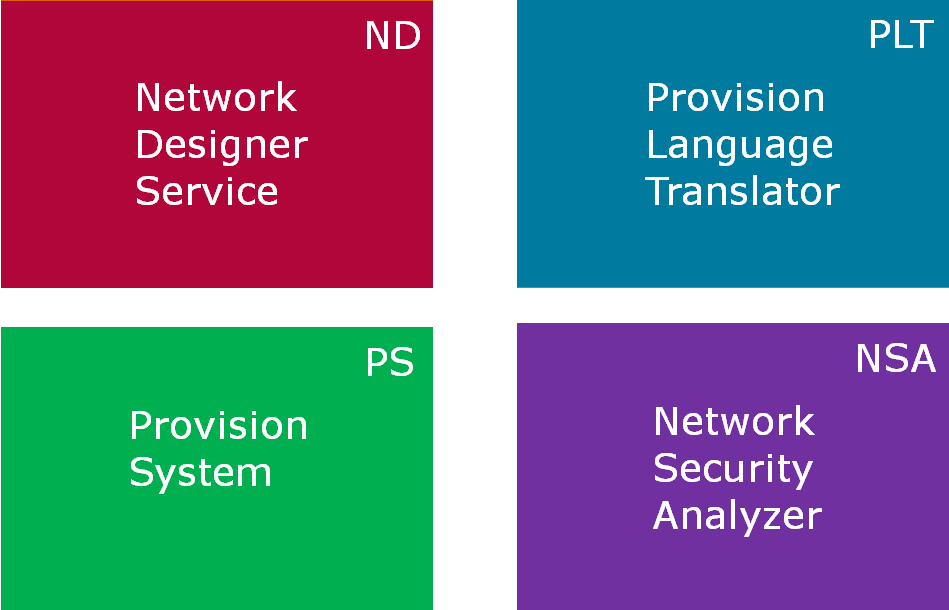
\includegraphics[width=145mm]{slg_structure.png}
\caption{Security Lab Generator}
\label{overflow}
\end{figure}

As it was mentioned above the concept supposed that all systems can be independently used. It supposed that must be some specified application programming interface (API) for communication between each other. Also it should provide the web user interface for convenient work. It is important to provide flexibility not only in communication between system, but also between modules inside the systems. It means that most of system must be able to extended by additional modules, functionality written by third-party developers. The main idea is combining any modules, systems, reusing some components to able to build needed custom project for solving different tasks.    


We just say that everything must be specified, but we do not talk how. It will be done on the stage of developing the architecture and it is out of scope of the report. So now it does not matter which protocol to use REST, SOAP or other and how to integrate the modules.


\section{\myNDS}
The purpose of the \myNDS{ }is to provide easy way to design the network including specifying networks, hosts, connections, software, user accounts. The system should provide the flexibility providing by IaaS and simplicity providing by PaaS. It the first part of the big ecosystem. The system should provide the capability to export designed network as structured data. For example XML, JSON or other. It could be used independently by system administrator to design the network and collaboration. And also it can be used in combination with others system to perform the whole life cycle flow. As we mentioned in the previous subsection we want to create project for automation of research. So it is the first step to reach goal. 

On the Figure 2 you can see the network topology of OpenStack. OpenStack is open source IaaS. As many IaaS OpenStack provide functionality to run any instances with any operation systems, creating any network structure. It is very flexible. As result of configuring the network and running the instances we can see the network topology describing the network.  It is quite easy to read. But IaaS does not provide simplicity of designing the network.     
\begin{figure}[ht!]
\centering
%[width=90mm]
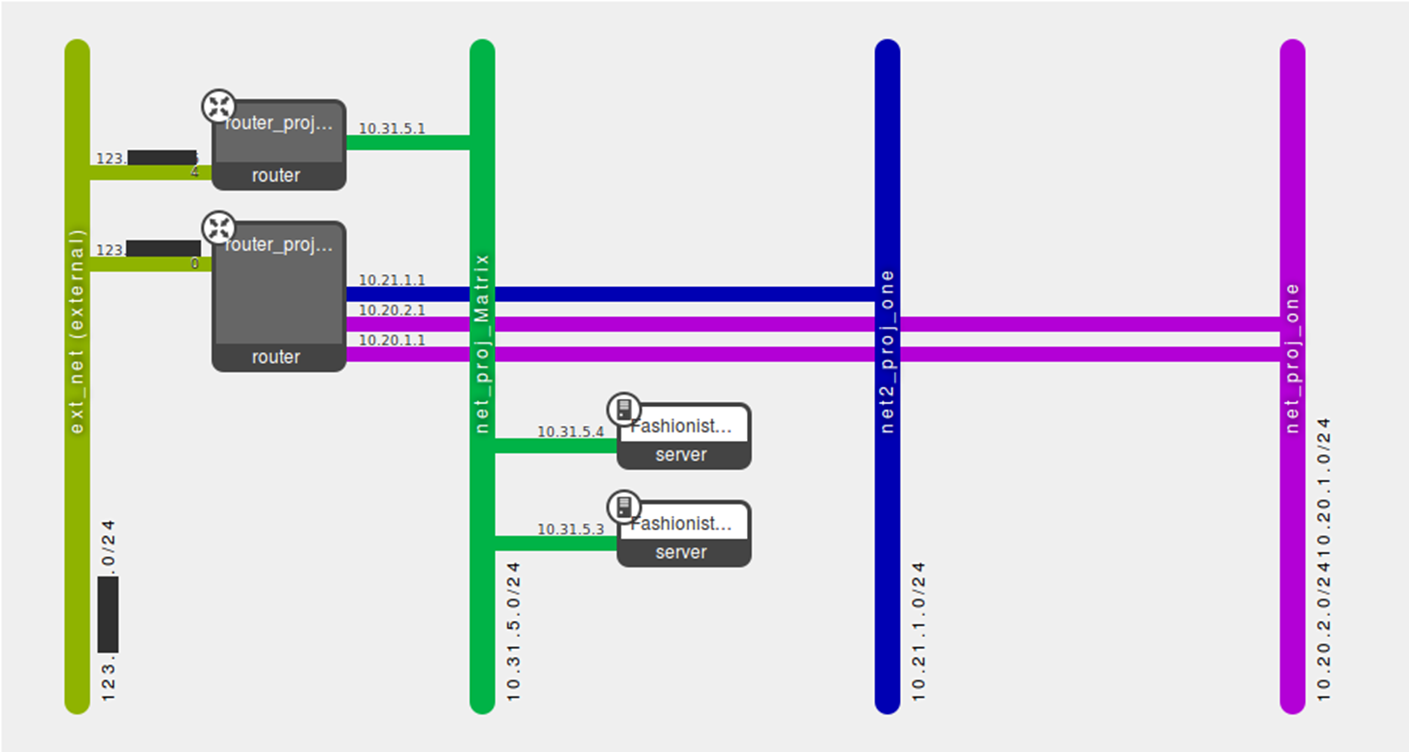
\includegraphics[width=145mm]{openstack_network_topology.png}
\caption{OpenStack network topology}
\label{overflow}
\end{figure}

On the other hand there are PaaS systems such as Jelastic, which admin console is illustrated on Figure 3. PaaS provide simplicity of designing. PaaS usually use already pre-defined network structure for different purposes such as Java applications, PHP, Ruby and so on. In this case administrators mostly do not care about orchestration the network structure, they care about which server to use, which database, needed if the load balancer or not and so on. 

The idea to combine two approaches from IaaS and PaaS to make flexible and simple designer to provide ability to create any complex network with specified hosts and specified installed software. 
     
\begin{figure}[ht!]
\centering
%[width=90mm]
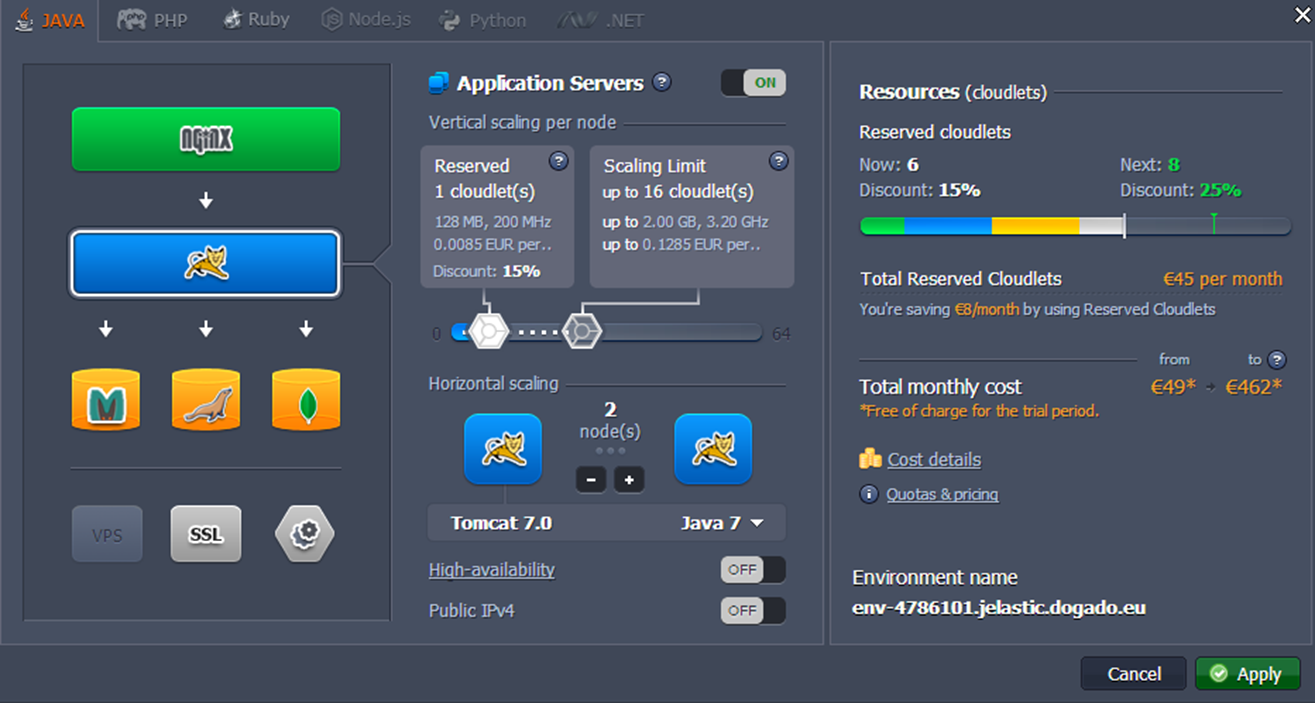
\includegraphics[width=145mm]{jelastic.png}
\caption{Jelastic admin console}
\label{overflow}
\end{figure}


Research questions:
\begin{compactitem}
\item How to fully describe the network structure as XML, JSON or by other language with ability  to use the it as a provision language?
\item How to specify the principle of network designer for complex structure by combining flexibility IaaS and simplicity PaaS constructor?  
\end{compactitem}


\section{\myPLT}
Some system provide the capability to describe the environment and deploy it. But each system has its own language. If you do not need to use different provision providers then there is not problem. But it could be that you will need to migrate from one provider to other. For example from Amazon Web Service (AWS) to your own server with VMware EXSi. In this case you have to spend a lot of time to deploy the same environment on your own servers. To automatize the process you would like to use some tools like Vagrant, but it can not resolve all problems of migration, because you still have to write instructions for Vagrant manually. To overcome the problem of migration and provide flexibility in choosing the provider for deploying the environment, we suggest the concept of Provision Language Translator (PLT). 


PLT is a translator like Google Translator, but not for nature languages. It is a translator for provision languages. Provision language is a full description of the environment that cloud be used for deploying described environment according to the description. Idea of PLT is to provide so many module as possible for bi-direction translation provision language. The project could be used independently by system administrators for migration network environments from on to other provision provider. But in our case we want to use it in combination with other systems. So we should provide the translation from our network description language to already existing language like Vagrant file or Amazon Cloud Formation or others. So now we have 2 systems ND and PLT. We could design the network, export SLG XML and then translate it into the appropriate provision language. 

\begin{figure}[ht!]
\centering
%[width=90mm]
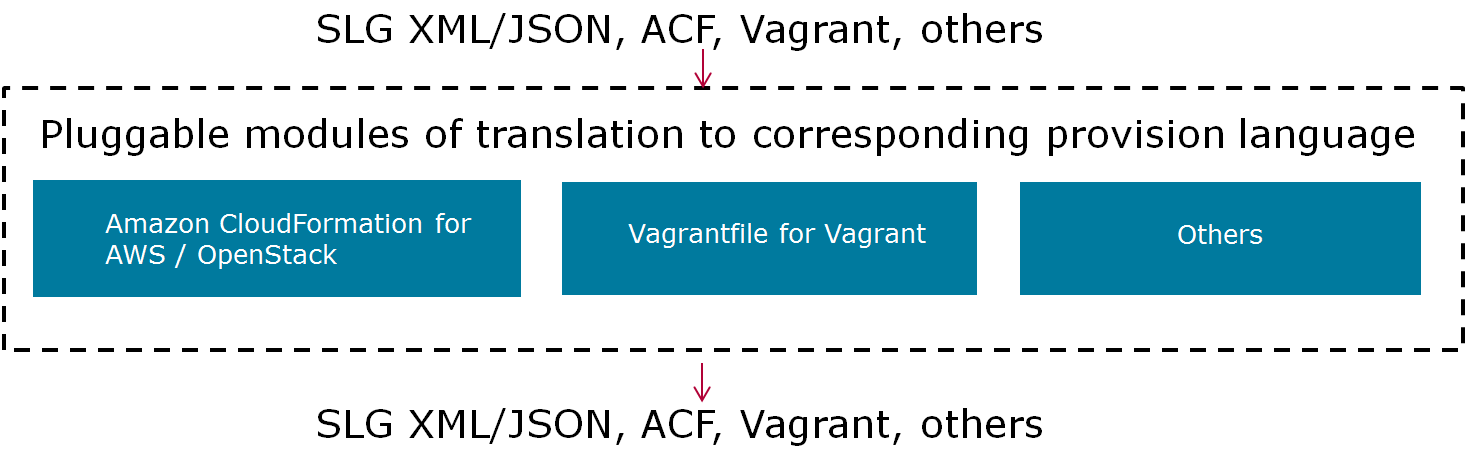
\includegraphics[width=145mm]{plt.png}
\caption{Provision language translator}
\label{overflow}
\end{figure}
     
Research questions:
\begin{compactitem}
\item How to convert/translate different provision languages in both direction saving the all structure?
\end{compactitem}  

\section{\myPS}
Provision system is used for deploying the environment based on the description. It can accept different types of provision language and provide provision on different providers: AWS, OpenStack, VMware, VirtualBox and so on. Provision system can directly apply provision language to provider or you can use PLT service to translate input provision language to appropriate for certain provider and then apply it. In combination of three described system we could design the network, convert to appropriate provision language and apply to certain provider. 

\begin{figure}[ht!]
\centering
%[width=90mm]
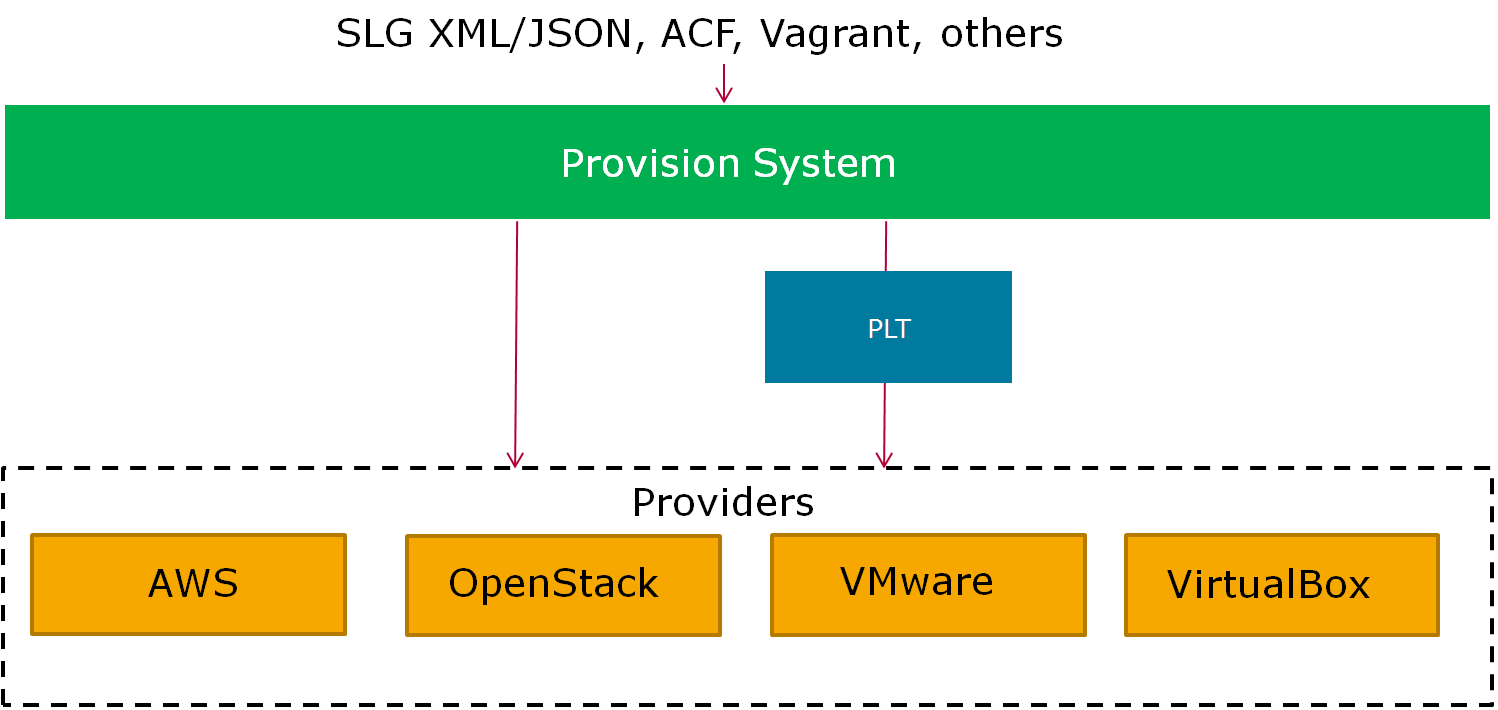
\includegraphics[width=145mm]{ps.png}
\caption{Provision system}
\label{overflow}
\end{figure}

Research questions:
\begin{compactitem}
\item How to implement orchestration tool for provision on the different providers? 
\end{compactitem}


\section{\myNSA}
Network system analyzer is the most interesting part of the project, because it is used for making research, gathering data from host, scanning the hosts, analyze data, making report and applying user scenarios. The system contains two parts: server side and agents. 

The server side is wrapper of many security analytic tools such as MulVal. All tools need data to analyze them and create reports, attack graph and show some statistics. So server must know about the whole network structure also gather data from the hosts. The first issue could be solved by passing the SLG XML describing designed network from Network Designer. Already on this step NSA can provide some information such as an attack graph and potential vulnerabilities. But is is not enough. We need information about hosts. For this issue we can use agent. 

The NSA agent is client side application. The agent could include different inventory, monitoring, suffering tools to make fully analyzing of the host. Some of possible tools: OVAL SCANNER, NESSUSS and others !!!!. The agent registers in the server and ready to send data to server. The server receive data and depending on the data delegates them to the appropriate analytic tool. The system could get access to other services that could provide useful information for making reports and analyzing data. For example the system could work with Vulnerability Database (VDB) or RAIMS???!!!

Other very important purpose is creating custom user scenarios, send them to agent and agent apply them. Firstly the concept implies that users can create some description of user scenarios which must be performed on the host side. User scenarios could be some activities such as login,logout, run service, install software, open connections, create files and so on. The NSA must provide the mechanism of simple way of implementation any user scenarios for any operation system. The scenarios must be packed as cookbook (analogy to cookbooks for Chef). It is implied that we will have the repository with set of pre-defined reusable cookbooks. Any user can create his own cookbook, reuse some repository, include his cookbook to repository and combine any cookbooks. 

The server takes cookbooks with user scenarios and apply them to host by agents that must be installed on the hosts. As it is just concept we do not distinguish agents by purposed, but we can expect that functionality of gathering data and applying cookbooks could be distributed into different application. But any way both of them are agents and they are installed on the hosts.         

\begin{figure}[ht!]
\centering
%[width=90mm]
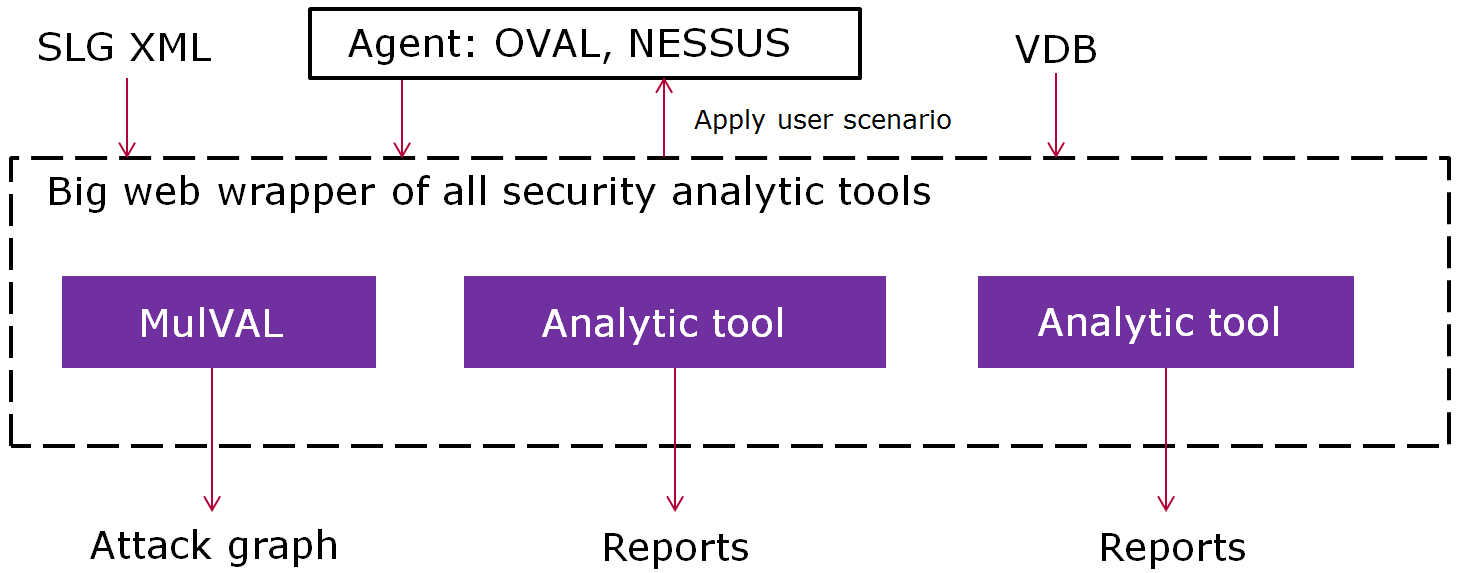
\includegraphics[width=145mm]{nsa.png}
\caption{Network Security Analyzer}
\label{overflow}
\end{figure}

Research questions:
\begin{compactitem}
\item How to collect all information about the host by special agent wrappers different monitoring tools?  
\item How to normalize collected data to use them for analyzing?  
\item How to analyze data?
\item How to create reports according collected data and analyzed data? 
\item How to applying scenarios to hosts. 
\item How you describe the user scenarios to be able to reuse them and combine with others?
\end{compactitem}

\section{Conclusion}

To conclude let's remember the main points. In this report we mentioned some problems of researchers that make overhead of the research. The main overhead is because of the preparation stage including creation the research network environment, configuration the network and hosts, installation software, generating data, simulation some typical events. In the report we suggest the concept of the project that can probably solve some of the problems and overcome in some cases the research overhead. We suggest module structure of the project that implies that the project consists of several independent system. And every system can be used independently by administrators, users, researchers or in combination with others.     

To prove the idea of concept we gave some usecases of using every system and the whole project. As it is research project we consider possible research questions and ares for researching during the developing the system as a prove of the concept. 
%------------------------------------------------

\section{Methods}

Maecenas sed ultricies felis. Sed imperdiet dictum arcu a egestas. 
\begin{compactitem}
\item Donec dolor arcu, rutrum id molestie in, viverra sed diam
\item Curabitur feugiat
\item turpis sed auctor facilisis
\item arcu eros accumsan lorem, at posuere mi diam sit amet tortor
\item Fusce fermentum, mi sit amet euismod rutrum
\item sem lorem molestie diam, iaculis aliquet sapien tortor non nisi
\item Pellentesque bibendum pretium aliquet
\end{compactitem}
\lipsum[4] % Dummy text

%------------------------------------------------

\section{Results}

\begin{table}[H]
\caption{Example table}
\centering
\begin{tabular}{llr}
\toprule
\multicolumn{2}{c}{Name} \\
\cmidrule(r){1-2}
First name & Last Name & Grade \\
\midrule
John & Doe & $7.5$ \\
Richard & Miles & $2$ \\
\bottomrule
\end{tabular}
\end{table}

\lipsum[5] % Dummy text

\begin{equation}
\label{eq:emc}
e = mc^2
\end{equation}

\lipsum[6] % Dummy text

%------------------------------------------------

\section{Discussion}

\subsection{Subsection One}

\lipsum[7] % Dummy text

\subsection{Subsection Two}

\lipsum[8] % Dummy text

%----------------------------------------------------------------------------------------
%	REFERENCE LIST
%----------------------------------------------------------------------------------------

%\begin{thebibliography}{99} % Bibliography - this is intentionally simple in this template
%
%\bibitem[1]{Figueredo:2009dg}
%Figueredo, A.~J. and Wolf, P. S.~A. (2009).
%\newblock Assortative pairing and life history strategy - a cross-cultural
%  study.
%\newblock {\em Human Nature}, 20:317--330.
% 
%\end{thebibliography}

\input{mylib.bbl}
\bibliographystyle{IEEEtran}
%\bibliographystyle{ieeetr}
\bibliography{mylib}


%----------------------------------------------------------------------------------------

% Multicolumn END
%\end{multicols}

%\bibliography{mylib}

\end{document}
